\chapter{Choix de développement}

\section{Les métadonnées}
\subsection{Utilisation des métadonnées stockées sur le disque dans le code
source de GELI}
\label{ssec:md_usage}
L'analyse de \textit{LUKS} et \textit{GELI} nous a montré les similitudes et
différences que présentent ces deux systèmes.
\paragraph{}
\begin{figure}[h]
\centering
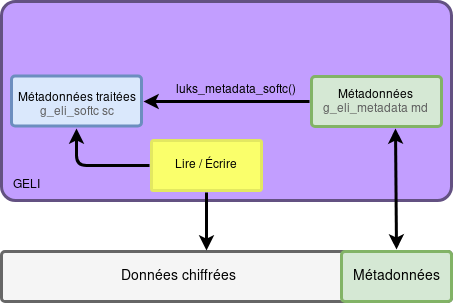
\includegraphics[width=.6\linewidth]{choix_developpement/utilisation_metadonnee.png}
\caption{\label{fig:softc_eli}Métadonnées en mémoire}
\end{figure}

\paragraph{}
Pour n'importe-quel module noyau utilisant la classe \textit{GEOM} de
\textit{FreeBSD}, les métadonnées sont toujours placées à la fin des données du
disque, contrairement à \textit{LUKS}. Il faut donc créer les fonctions
utilisant celles fournies par \textit{GEOM} afin de réaliser cette opération.
\paragraph{}
Dans le cas d'un fichier (utile pour sauvegarder l'en-tête contenant les 
métadonnées), il suffit d'utiliser les fonctions standards de
\verb|C| et de lire le début du fichier. Dans le cas d'un disque en revanche, il
faut créer une fonction lisant les premiers secteurs. On peut ensuite les
stocker dans une structure afin de connaître les propriétés de chiffrement
utilisées.

\paragraph{}
Les informations présentes dans les métadonnées \textit{LUKS} sont assez proches
de celles de \textit{GELI}:
\begin{itemize}
\item le \textit{MAGIC}
\item la version utilisée
\item l'algorithme de chiffrement
\item l'algorithme de hashage
\item le sel
\item le nombre d'itérations PKCS
\item la \textit{masterkey} chiffrée
\end{itemize}

\paragraph{}
Les métadonnées sont donc stockées sur le disque et sont mappées en mémoire via
la structure {\em md} de type {\em g\_eli\_metadata}. Mais des métadonnées 
"indirectes" sont aussi présentes en mémoire à travers la structure {\em softc} 
de type {\em g\_eli\_softc}. Comme illustré par le schéma \ref{fig:softc_eli} 
cette structure diffère des 
métadonnées à proprement parler. En effet les métadonnées évoquées jusqu'ici sont
celles qui sont stockées telles quelles sur le disque à l'encodage près. Les 
données privées de l'instance GEOM sont stockées dans une structure présente 
uniquement en mémoire et dont les champs sont remplis par les métadonnées du 
disque, mais aussi par des informations sur le disque comme sa taille ou encore 
la taille des secteurs. Enfin les clés de chiffrement qui sont dérivées à partir
de la clé maître y sont également stockées sous la forme d'un arbre et d'une 
queue.

\subsection{Transformer les métadonnées de LUKS en métadonnées GELI}
\subsubsection{Principe général}
\paragraph{}
Écrire un module noyau de toute pièce capable d'utiliser un disque chiffré avec
\textit{LUKS} serait une tâche très longue. Sachant que de nombreuses fonctions
s'inspireraient du module \textit{GELI}, il est préférable de copier le code
(sous license \underline{BSD-2-Clause-FreeBSD}) et de l'adapter à la lecture et
l'écriture de données sur un disque chiffré \textit{LUKS}. Cependant, les
fonctions étant extrêmement dépendantes de la structure des métadonnées, 
que ce soit directement ou à travers la structure {\em softc} (qui 
désigne les données privées de l'instance GEOM), leur
modification équivaudrait à une refonte assez importante du code.
\paragraph{}
\begin{figure}[h]
\centering
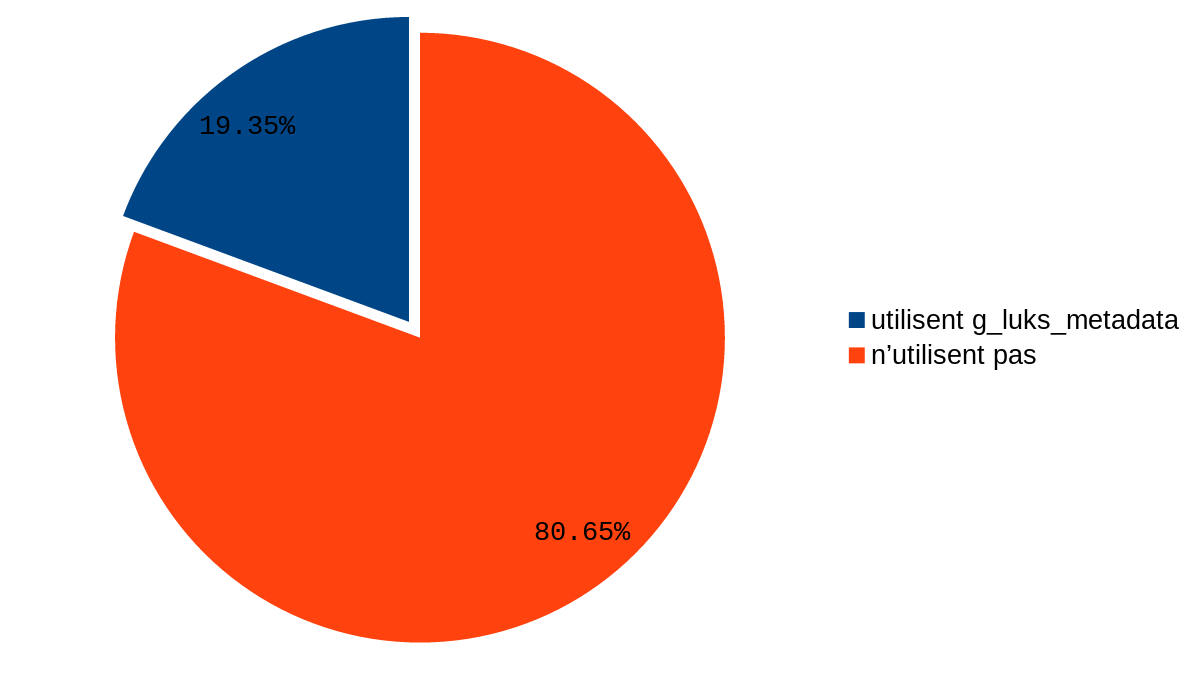
\includegraphics[width=.9\linewidth]{choix_developpement/fonctions_g_luks_metadata.png}
\caption{\label{fig:fonctions_md}Fonctions utilisant les métadonnées}
\end{figure}
\paragraph{}
\begin{figure}[h]
\centering
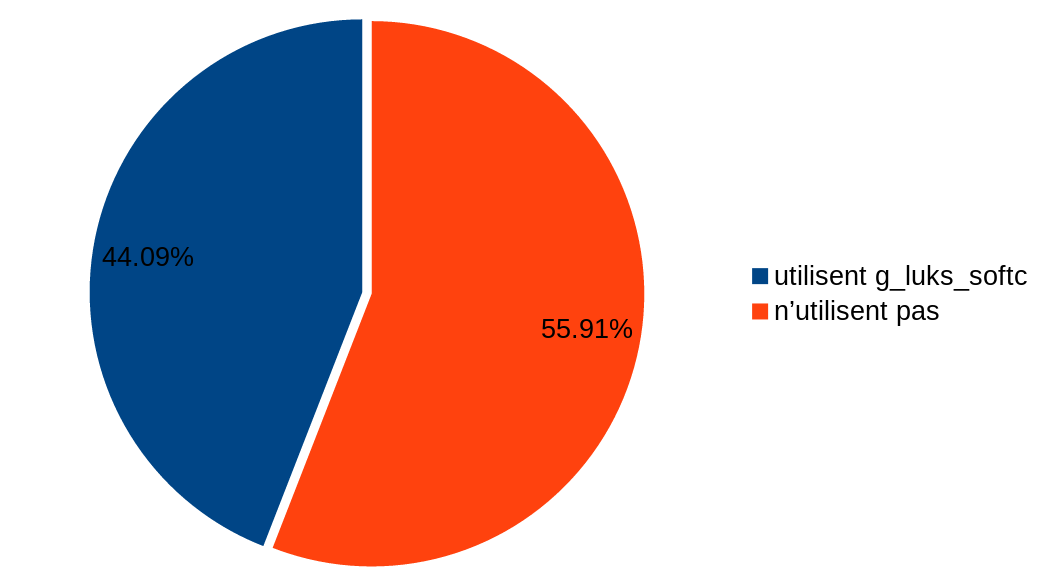
\includegraphics[width=.9\linewidth]{choix_developpement/fonctions_g_luks_softc.png}
\caption{\label{fig:fonctions_sc}Fonctions utilisant la structure \texttt{softc}}
\end{figure}
\paragraph{}
C'est pourquoi, la solution la plus intéressante serait de garder la structure
de \textit{GELI} et d'y mettre les informations de chiffrement. Cela permettra 
notamment d'écrire et/ou de modifier moins de code et donc de limiter les erreurs
et de faciliter la maintenabilité. De plus en choisissant de procéder ainsi, on
peut modifier le code facilement par itérations en le gardant compilable et 
exécutable. On choisit donc de conserver le code de 
GELI le plus possible et de transformer les métadonnées de LUKS en métadonnées 
GELI.

\paragraph{}
En effet bien que les métadonnées stockées sur le disque soient différentes 
entre GELI et LUKS, le chiffrement du disque reste essentiellement identique :
on utilise une clé maître et un algorithme de chiffrement de blocs. Cependant 
comme décrit auparavant, la clé maître dans GELI est dérivée en clés de 
chiffrement. Toutefois, GELI laisse la possibilité à travers des {\em Flags} 
d'utiliser la clé maître comme unique clé de chiffrement.

\paragraph{}
Comme décrit en \ref{ssec:md_usage}, les métadonnées utilisées par l'instance
GEOM sont celles qui sont stockées dans la stucture {\em softc}, à l'exception
de la lecture sur disque des métadonnées et de leur vérification ainsi que le 
changement des métadonnées sur le disque (changement de la phrase de passe et
donc de la clé chiffrée sur le disque).

\paragraph{}
\begin{figure}[h]
\centering
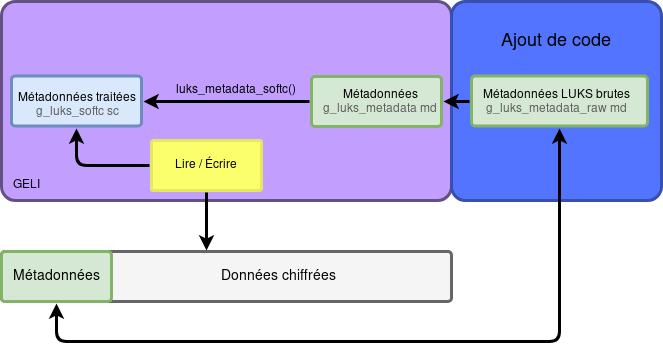
\includegraphics[width=.9\linewidth]{choix_developpement/utilisation_metadonnee_luks.png}
\caption{\label{fig:transformation_md}Transformation des métadonnées}
\end{figure}

\paragraph{}
La transformation des métadonnées LUKS en métadonnées GELI consiste donc à 
remplacer la lecture des métadonnées du disque par GELI par celles de LUKS 
comme illustré par le schéma \ref{fig:transformation_md}. On change donc la 
fonction {\em luks\_metadata\_softc} pour qu'elle utilise les données extraites
de l'en tête LUKS du disque au lieu de celles extraites de l'en tête GELI, donc
respectivement du premier secteur et de quelques secteurs suivant au lieu du 
dernier secteur. On devra également changer la gestion du déchiffrement de la 
clé du disque.


\subsubsection{Déchiffrement de la clé de chiffrement dans le cas de GELI}
Dans le cas de GELI, le code prévoit le déchiffrement de la clé de chiffrement 
dans le noyau, de façon à pouvoir déchiffrer le disque au démarrage (pour 
pouvoir avec un volume racine chiffré). Plus précisément l'utilitaire en espace
utilisateur envoie au noyau via l'API de GEOM, la phrase de passe dérivée via 
l'algorithme PKCS5v2 en prenant SHA512 comme fonction pseudo aléatoire.


\subsubsection{Déchiffrement de la clé de chiffrement dans le cas de LUKS}
\paragraph{}
On a donc besoin de déchiffrer la clé de chiffrement stockée dans l'en-tête LUKS.
Pour cela il faut tout d'abord bien comprendre comment est stockée la clé de 
chiffrement sur le disque.

\paragraph{}
La clé de chiffrement est hashée selon l'algorithme spécifiée par le champ
{\em hash-spec}, et stockée dans le champ {\em mkdigest} (Master Key Digest).

L'en-tête LUKS permet de stocker la même clé chiffrée avec huits phrases de passe
différentes, dans les huits {\em KeySlot} définis par le standard.
\\
Pour un keyslot, la phrase de passe est dérivée selon l'aglorithme {\em PKCS5v2}
avec comme fonction pseudo aléatoire l'algorithme de hashage spécifié par 
{\em hash-spec}. La clé est ensuite fragmentée via l'algorithme 
{\em anti-forensic splitter} spécifié dans \cite{AFsplitting} qui a pour but de
lutter contre la persistance des informations stockées sur des disques dur
(disques qui utilisent le magnétisme pour stocker les données)
\\
Enfin le résultat de la fragmentation est chiffrée selon l'algorithme utilisé 
pour les données du disque (donc précisé par les champs {\em cipher-name} et 
{\em cipher-mode}) avec comme clé le résultat de la dérivation de la phrase de
passe.


